\section{Biblioteki}

\begin{frame}[t]\frametitle{Biblioteki statyczne}

  Biblioteka statyczna to archiwum plików ``relocatable'', więc korzysta się z
  niej analogicznie jak z tych plików. Nazwa takiej biblioteki zazwyczaj
  rozpoczyna się od 'lib' a kończy się rozszerzeniem ``.a''.

  Aby zbudować bibliotekę statyczną korzystamy z polecenia
  \fbox{gcc -static -o libfoo.a foo.o}

  Aby skorzystać z takiej biblioteki korzystamy z polecenia
  \fbox{gcc example.o -lfoo}
  
\end{frame}

\begin{frame}[t]\frametitle{kolejność linkowania}
  \begin{figure}
    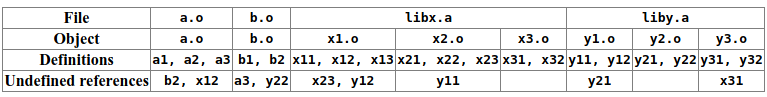
\includegraphics[width=\textwidth]{staticLib.png}
    \caption{zależności przy linkowaniu \cite{lurklurk}}
  \end{figure}
\end{frame}



\begin{frame}[t]\frametitle{Współdzielone (shared)}
  Aby stworzyć plik biblioteki współdzielonej musimy wywołać następującą komendę:
  
  \fbox{gcc -shared -o libfoo.so foo.o}

  jednak plik obiektowy foo.o musi być odpowiednio skompilowany ( flaga -fPIC )
  ponieważ pliki typu .so muszą być ,,position independent''

  [\url{przyklady/02_shared}]
\end{frame}

\subsection{Realocation and PIC}
\begin{frame}[t]\frametitle{Realocation vs Position Independent Code}
  \begin{alertblock}{Re alokacja} polega na wyliczeniu poprawnych adresów obiektów z biblioteki
    współdzielonej przed uruchomieniem programu.
  \end{alertblock}

  \begin{alertblock}{Position Independent Code} jest nowszą technologią która zakłada że poprzez
    dodanie warstwy abstrakcji sekcja .text ma uprawnienia tylko do odczytu, co
    zapewnia proste mapowanie adresów, zwiększa bezpieczeństwo i zapewnia
    współdzielenie kodu biblioteki przez wiele procesów
  \end{alertblock}
\end{frame}
\subsection{GOT}
\begin{frame}[t]\frametitle{Global Offset Table}
  \begin{figure}
    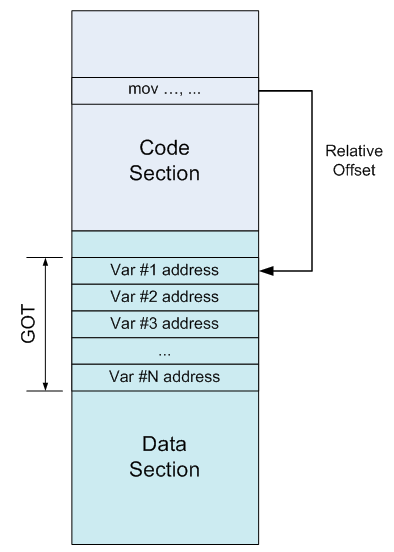
\includegraphics[height=0.65\textheight]{GOT.png}
    \caption{Schemat tablicy GOT\cite{PIC}}
  \end{figure}
  [\url{przyklady/PIC_variable/}]
\end{frame}
\subsection{PLT}
\begin{frame}[t]\frametitle{Procedure Link Table}
  \begin{figure}
    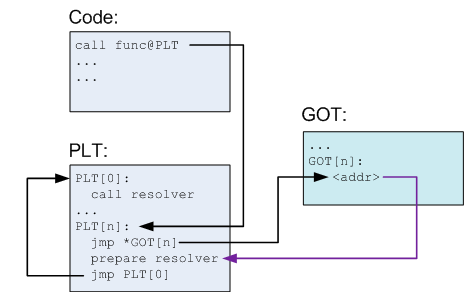
\includegraphics[height=0.65\textheight]{PLT.png}
    \caption{Schemat tablicy PLT przed pierwszym wywołaniem funkcji\cite{PIC}}
  \end{figure}
\end{frame}


\begin{frame}[t]\frametitle{Procedure Link Table}
  \begin{figure}
    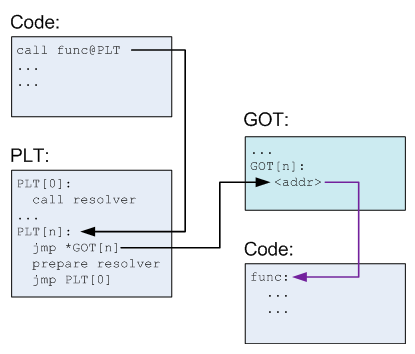
\includegraphics[height=0.65\textheight]{PLT1.png}
    \caption{Schemat tablicy PLT po pierwszym wywołaniem funkcji\cite{PIC}}
  \end{figure}
  [\url{przyklady/PIC_functions}]
\end{frame}

\subsection{Dynamiczne ładowanie bibliotek}

\begin{frame}[t]\frametitle{dlfcn.h}
 \cite{tldp} Biblioteka ``dlfcn.h'' umożliwia dynamiczne ładowanie bibliotek
  współdzielonych w trakcie działania programu
\newline
  Do obiektów biblioteki mamy dostęp poprzez handler zwracany z funkcji
  \fbox{void * dlopen(const char *filename, int flag);}
  \newline
  Do pierwszego argumentu można podać ścieżkę do pliku biblioteki
  współdzielonej, lub jej nazwę ( wtedy będzie szukana w domyślnych katalogach
  lub w LD\_LIBRARY\_PATH)
\newline
  Drugi argument określa czy linkowanie będzie leniwe, czy od razu z linkować
  wszystkie obiekty.
\newline
  \fbox{void * dlsym(void *handle, char *symbol);}
\newline
  Powyższa funkcja zwraca wskaźnik na obiekt którego żądamy w argumencie
  \newline
  [\url{przyklady/DL_library}]

\end{frame}
